\chapter{Introduction}
\label{chp:introduction}

\section{Definitions}

\emph{Augmented Reality (AR)} is seen on the Reality-Vitality (RV) Continuum a subsection of Mixed Reality (MR). The RV Continuum represents the degree of mixing up a picture representing the real environment with parts of the virtual environment. This mixed picture will be shown on one display. In contrast to a purely virtual environment picture, the so called virtual reality (VR), AR contains a big part of the real environment picture and some part of the virtual environment.
In their paper, \cite{Milgram1994AugmentedContinuum} define a more detailed framework for the taxonomy of those terms. (
differentiation of the different styles of mixed reality) TODO

With a head mounted Device it will be possible 

\begin{figure}[h]
    \centering
    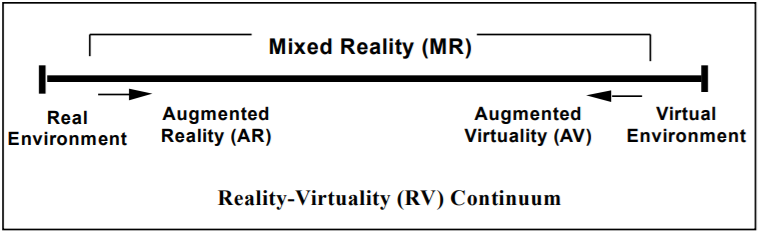
\includegraphics[width=0.95\textwidth]{RealityVirtualityContinuum}
    \caption{Simplified representation of a RV Continuum (from \cite{Milgram1994AugmentedContinuum})}
\end{figure}
\noindent
For simplicity for this work  a picture which is composed of a real image and a computer calculated image will be called an AR-image. The real image will be taken by the camera of a device. For the computation of the computer-generated image hints from the real image, such as a position anchor can be used. An example of an AR-image is a digital Object displayed in front of a real image background, e.g. a digital chess figure on a real table.

\emph{Google Cardboard} is a box mostly made out cardboard. It holds the head-mounted device e.g. a smartphone. Through a pair of lenses, serving as a magnifier, the viewer can see a split image in a way, such that each eye will just see its side of it and therefore a different picture. This enables a binocular vision which then produces a 3D effect.
Any sort of a box in the style of the Google Cardboard should be usable for this project. Important for this work is a hole in the front wall for the smartphone camera. 
\begin{figure}
	\begin{subfigure}[t]{0.45\textwidth}
		\centering
		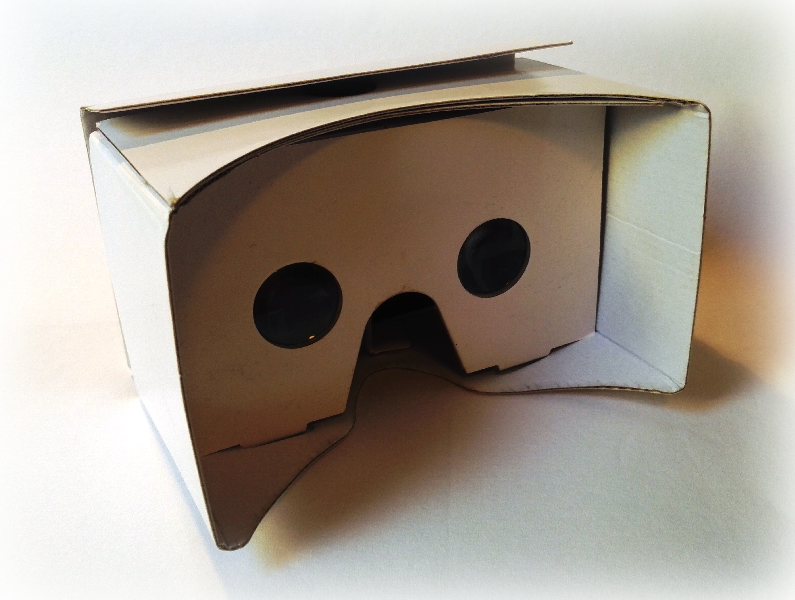
\includegraphics[height = 3.5cm]{GoogleCardboardRearView}
		\caption{}
	\end{subfigure}
	\hfill
	\begin{subfigure}[t]{0.45\textwidth}
		\centering
		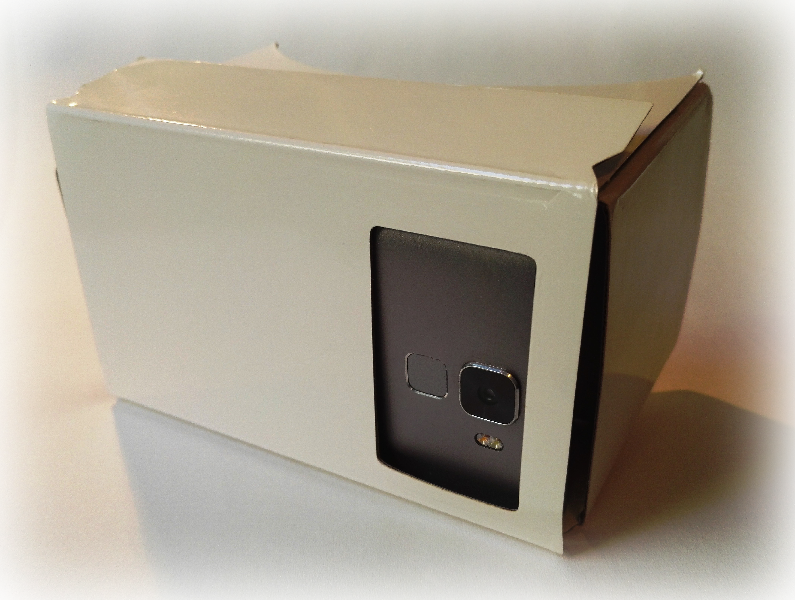
\includegraphics[height = 3.5cm]{GoogleCardboardFrontView}
		\caption{}
	\end{subfigure}
	\caption[Google Cardboard with smartphone]
			{(a) Google Cardboard rear view where the two lenses are located.
			 (b) Google Cardboard front view with the spare hole for the smartphone camera.}
\end{figure}


\section{Motivation}

Over the past years VR, AR and MR became very popular. There are a lot of application for VR, which works quite simple whit a smartphone and the so-called Google Cardboard. With the same principle and the inclusion of the device camera exists also application for augmented reality. Each of those application must be developed for a certain operation system concerning the specific integration of hardware and software. 
The use of web technology, more concrete a web browser with the necessary API to use camera and some sort of GPU or even other useful features, could overcome the cap of the different operating systems. On one hand, it would ease the use and accessibility of such a web application, as no other application must be installed than a browser with the traits aforementioned. On the other hand, developing such an application would have the same nice restriction and advantages. 



\section{Goal, outline and approach}

The main focus of this projects lays on the creation of an AR-demo for Google Cardboard based on JavaScript code and existing libraries. A secondary focus lays on testing some web based technology.
The goal will be approached in the following steps:

\begin{enumerate}
    \item In chapter 2As the digital part is quite crucial, it will be important to examine the feasibility of creating and understand the basics. A further evaluation of the means will show, whether a robust basis can be provided for the coming steps.
    
    Set up and test a rendering library on top of WebGL  - Either three.js, or develop your own (port jrtr from the computer graphics course, for example) 
    
    \item The inclusion of the camera is also a highly important part. At this stage of the project, the decision will be made, whether the intended library firstly can be implemented and secondly provides the means intended to create a demo.
    Set up and test an AR library 
    
    \item In the end it is about to combine knowledge and code from the first two steps and tweak the code, that it is compatible to use for the Google Cardboard and evaluated the usability of use and development.
\end{enumerate}


test libraries, show alternatives

Beside web based environment will be tested.

just to mention, for the documentation shareLatex is used.

Everything is made with using nothing than a browser. There are some nice online editors to program codes. For this project, the only editor Cloud9 from Amazon (Todo some references, Cloud9 IDE, LLC) 
see: https://aws.amazon.com/de/
was used. It has an integrated GitHub synchronisation and provides a server to execute and test the application directly.



Goal \& Description\\
Develop an augmented reality demo using Google Cardboard based on JavaScript code and existing libraries. Augmented reality includes using input devices (camera, hand tracker) to track real objects, modify/"filter" real images, render and manipulate virtual objects over the real background, enhance scene (textures, videos), or 3d reconstruction.

Reason: The idea is, that there is an easy access for all people with almost no effort of presettings.






\section{Requirements}

For this project the following list is needed to achieve an AR application:
\begin{itemize}
    \item Server to run the code
    \item Engine to process and calculates the digital part
    \item Access to the smartphone camera and provider for the real environment imagery
    \item Display on which the results of the two aforementioned points are merge and shown.
\end{itemize}

For displaying and process, I rely on libraries which use JavaScript and WebGL. As alternative there would be Flash or 2dCanvas.

test for WebGL support visit https://get.webgl.org/



Requirements and technical evaluation
API for WebGl
API for Camera
Possible any API for other features like microphone
At a very basic level of understanding/abstraction, the device need to provide a camera for capturing a image of the real world and a browser in which the computation and display part will be executed. 
Chrome supports those desired feature (some table which show that) and provides a nice building debugging tool for JavaScript. For this reason, this project will mainly be tested and developed in chrome and as a smartphone, an android with the version 6.0. It will be possible, that specific problems could occur for the testing devices.


\section{Background}


Base and related work
ThreeJs
And others






